% TEMPLATE for Usenix papers, specifically to meet requirements of
%  USENIX '05
% originally a template for producing IEEE-format articles using LaTeX.
%   written by Matthew Ward, CS Department, Worcester Polytechnic Institute.
% adapted by David Beazley for his excellent SWIG paper in Proceedings,
%   Tcl 96
% turned into a smartass generic template by De Clarke, with thanks to
%   both the above pioneers
% use at your own risk.  Complaints to /dev/null.
% make it two column with no page numbering, default is 10 point

% Munged by Fred Douglis <douglis@research.att.com> 10/97 to separate
% the .sty file from the LaTeX source template, so that people can
% more easily include the .sty file into an existing document.  Also
% changed to more closely follow the style guidelines as represented
% by the Word sample file. 

% Note that since 2010, USENIX does not require endnotes. If you want
% foot of page notes, don't include the endnotes package in the 
% usepackage command, below.

% This version uses the latex2e styles, not the very ancient 2.09 stuff.
\documentclass[letterpaper,twocolumn,10pt]{article}
\usepackage{uflru,epsfig,endnotes}
\usepackage{indentfirst}
\usepackage{kotex} % (UTF-8)
\usepackage{graphicx}
\usepackage{cite}
\DeclareGraphicsExtensions{.pdf,.png,.jpg}
\begin{document}

%don't want date printed
\date{}

%make title bold and 14 pt font (Latex default is non-bold, 16 pt)
\title{\Large \bf UFLRU: 비휘발성 메모리와 플래시 메모리의 계층 구조를 위한 영속 객체 스와핑 알고리즘}

%for single author (just remove % characters)
\author{
{\rm Yeonjin Noh}\\
Hanyang University
\and
{\rm Jinsoo Yoo}\\
Hanyang University
\and
{\rm Seongjin Lee}\\
Hanyang University
\and
{\rm Youjip Won}\\
Hanyang University
} % end author

\maketitle

% Use the following at camera-ready time to suppress page numbers.
% Comment it out when you first submit the paper for review.
\thispagestyle{empty}


\subsection*{요약} 
프로세스가 생성한 영속 객체를 비휘발성 메모리에 저장함으로써, 비휘발성 메모리의 낮은 입출력 지연을 이용하여 영속 객체를 생성 및 관리할 수 있다. 비휘발성 메모리는 낸드 플래시 메모리 또는 하드디스크에 비하여 적은 용량을 갖는 제약이 있다. 본 논문에서는 비휘발성 메모리와 낸드 플래시 메모리 간의 계층 구조를 통해서 낸드 플래시 메모리를 비휘발성 메모리의 스왑 영역으로 사용한다. 이와 같은 계층 구조를 사용함으로써 프로세스가 생성할 수 있는 영속 객체의 총 용량을 확장 시킨다. 이를 위해서, 스왑 영역으로 옮길 희생 영속 객체를 선택하는 UFLRU (Unmapped-object First LRU)알고리즘을 개발하였으며, CFLRU 알고리즘 대비 약 15\%의 성능 향상을 확인하였다.

\section{서론}
비휘발성 메모리 (Non-Volatile Memory)는 바이트 단위의 입출력 동작, DRAM과 유사한 수준의 입출력 지연, 그리고 데이터의 영속적인 저장과 같은 장점을 가지는 차세대 저장장치이다. 비휘발성 메모리로는 Spin-torque transfer RAM (STT-RAM), Phase change memory (PCM), Resistive RAM (ReRAM) 등이 있다. 이러한 비휘발성 메모리를 프로세스 주소공간의 영속 객체\cite{}를 저장하기 위한 메모리로 사용하는 연구들이 제안되어 왔다 \cite{Memosyne}\cite{hwang2015heapo}\cite{others}. 이들 연구에서는 프로세스 주소공간의 영속성을 갖는 객체들을 블록 디바이스 (HDD, SSD)가 아닌 비휘발성 메모리에 저장함으로써, 블록 기반 입출력 overhead를 제거하고 시스템의 성능을 향상시킨다. HEAPO\cite{HEAPO}의 경우, 프로세스의 가상 주소공간에 영속 힙 (persistent heap)을 만들고, 해당 주소 공간을 비 휘발성 메모리의 물리 주소에 binding 함으로써 영속 힙의 객체들에게 영속성을 부여하였다.

HEAPO의 이러한 영속 객체 관리 기법은 CPU가 비휘발성 메모리를 직접 접근할 수 있도록 함으로써, 비휘발성 메모리가 갖는 낮은 입출력 지연, Byte addressibility 등의 장점을 시스템이 충분히 활용할 수 있도록 한다. 그러나 프로세스의 영속 힙 공간을 비휘발성 메모리에 1:1로 binding 함으로써, 프로세스가 생성할 수 있는 영속 객체의 수가 비 휘발성 메모리의 크기에 제한된다는 한계를 갖는다.

본 논문에서는 이러한 한계점을 해결하기 위해, 비휘발성 메모리와 플래시 메모리의 계층 구조를 구성하고, 비휘발성 메모리에 영속 객체를 할당할 공간이 부족할 경우, 비휘발성 메모리의 영속 객체를 낸드 플래시로 방출하는 스왑 인/아웃 기법을 적용한다. 이러한 기법을 통해 프로세스가 생성할 수 있는 영속 객체의 총 용량을 확장한다. 또한, 스왑 영역으로 옮길 희생 영속 객체를 선택하는데에 최적화 된 희생 페이지 선택 알고리즘인 UFLRU (Unmapped-object First LRU) 알고리즘을 개발하였으며, CFLRU \cite{park2006cflru} 알고리즘 대비 약 15\%의 성능 향상을 확인하였다.

\section{배경}
\subsection{비휘발성 메모리}
(작성)
\subsection{영속 객체 힙 저장소(HEAPO)}
영속 객체 힙 저장소 (Heap-Based Persistency Object Store) \cite{hwang2015heapo}는 프로세스의 가상 주소 공간 중 일정 영역을 할당 받아 영속 객체를 위한 주소 영역으로 사용하는 기법이다. 영속 객체를 저장하는 프로세스의 주소 영역을 영속 객체 힙이라 한다. HEAPO는 프로세스에게 영속 객체 힙 영역을 사용할 수 있는 인터페이스를 제공하며, 프로세스는 이러한 인터페이스를 통해서만 영속 객체 힙에 영속 객체를 생성 및 관리를 할 수 있다. HEAPO에 생성된 영속 객체는 시스템의 비 휘발성 메모리에 저장되어, 시스템 종료 시에도 데이터의 영속성을 보장받게 된다. 또한, HEAPO에서는 각 프로세스가 생성하거나 변경 한 영속 객체에 대한 정보를 영속 객체 힙 영역에 반영하여, 같은 영속 객체를 공유하는 프로세스에게 동일한 정보를 제공할 수 있다. 

영속 객체 가상 주소 영역은 HEAPO에서 관리되며, 비 휘발성 메모리의 물리 주소와 1:1로 대응 된다. 이를 위해, HEAPO는 영속 객체의 가상 주소 영역에 대응 되는 물리 주소들을 저장하고 관리한다. 이러한 구조는 프로세스가 영속 객체에 대한 가상 주소를 통해서 그에 대응하는 물리 주소를 얻을 수 있도록 해주는 역할을 하게 된다. 때문에, 프로세스는 영속 객체에 가상 주소만 있다면 영속 객체의 물리 주소를 얻을 수 있게 된다. 이를 위해, 프로세스는 HEAPO가 관리 중인 영속 객체의 가상 주소 영역을 프로세스 자신의 주소 영역으로 복사하며, 이러한 과정을 매핑 (Mapping)이라 부른다. 

이 후, 영속 객체가 매핑 된 프로세스가 영속 객체에 접근할 때, 물리 주소에 대한 정보가 없으므로 페이지 폴트가 발생하게 된다. 페이지 폴트 과정 중, 프로세스는 페이지 폴트가 일어난 가상 주소 영역에 대응 되는 물리 주소를 HEAPO로부터 반환 받게 된다. HEAPO의 이러한 1:1 대응 메모리 관리 방법은 허가 받지 않는 프로세스의 영속 객체 접근을 제한하는 것은 물론, 다수의 프로세스에 의한 영속 객체의 공유 기능을 제공한다.

현재 HEAPO에서는 메모리의 용량이 부족할 때 추가적인 메모리를 확보하는 정책이 없다. 때문에, 비 휘발성 메모리의 물리 주소를 모두 할당한 경우에는, HEAPO에서 추가적인 영속 객체의 할당이 불가능하게 된다. 즉, HEAPO의 총 영속 객체의 크기가 비 휘발성 메모리의 크기에 한정되는 문제점이 발생하게 된다는 것이다. 이를 해결하기 위해서는 스왑 인/아웃과 같은 메모리 확보 정책을 통해 추가적인 메모리를 확보하는 과정이 반드시 필요하다. 본 논문에서는 이를 위해, 비 휘발성 메모리와 낸드 플래시 간의 계층 구조를 구성하여, 비 휘발성 메모리의 용량이 부족할 경우 스왑 인/아웃 기법을 통해 영속 객체를 낸드 플래시에 기록하여 추가적인 메모리를 확보하고자 한다. 

HEAPO에서 영속 객체를 할당할 때는 malloc() 함수를 사용하며, 이는 영속 객체에 대한 메타데이터 또한 마찬가지이다. 때문에, HEAPO에서의 모든 물리 페이지들은 익명 페이지 (Anonymous page)로 취급 되어 비 휘발성 메모리에 기록된다. 때문에, HEAPO의 비 휘발성 메모리의 In/Active list에는 익명 페이지만 존재하며, 기존 리눅스와는 달리 파일 기반 페이지 (File Based Page)에 대한 처리나 검사가 불필요하다. 때문에, HEAPO에서의 스왑 인/아웃을 구현할 때는 파일 기반 페이지의 처리보다는, 익명 페이지에 대한 처리에 대한 계획을 주안점으로 두어야 할 것이다. 

또 다른 고려 사항은, HEAPO와 프로세스 간의 물리 메모리 Consistency이다. 메모리 확보 기법을 통해 영속 객체의 물리 주소를 변경할 경우, 프로세스와 HEAPO 간의 Consistency를 고려해 주어야 한다. 이를 위해서는, HEAPO의 물리 주소가 변경 되는 경우, 해당 물리 주소를 참조하는 모든 프로세스들을 검색하여 정보를 갱신하는 작업이 필요하다. 문제는, 이러한 프로세스의 검색 및 수정에 의한 성능 저하가 매우 크다는 점이다. 때문에, HEAPO에서 스왑 인/아웃을 구현할 때는 확보할 메모리의 매핑 여부를 고려해야 하며, 매핑이 되어있지 않은 페이지를 우선적으로 메모리 확보 대상으로 선정해야 한다.

\subsection{리눅스의 스왑 정책}

리눅스는 할당된 물리페이지를 2 종류의 LRU 리스트로 관리하며, 이는 각각 Active list 와 Inactive list이다. 페이지는 접근빈도에 따라 Active list와 Inactive list 간을 이동하며, 최근에 빈번하게 접근된 페이지는 active list에, 사용된 지 오래된 페이지는 inactive list에서 관리된다. 페이지는 이와 관련하여 2개의 Flag를 가지며, 이는 각각 PG\_active  Flag와 PG\_referenced Flag 이다. PG\_active Flag는 페이지가 어떤 list에 있는지를 나타내며, set 되어 있을 경우 해당 페이지는 Active list에, reset 되어 있을 경우 해당 페이지는 Inactive list에 있음을 의미한다. PG\_referenced Flag는 페이지의 접근 빈도를 나타내며, 0또는 1의 값을 갖는다. 이 값은 페이지가 프로세스에 의해 접근될 때, 또는 swap out의 victim 선정과정에서 변경된다. 

할당된 페이지는 먼저 Active list에 삽입한다. 이 때 페이지의 reference (PG\_referenced) 값은 0으로 설정된다. 페이지가 프로세스에 의해서 접근될 때마다 reference 값은 0에서 1로 변경된다. 만일 접근한 페이지의 reference 값이 이미 1이고, 해당 페이지가 현재 Inactive list에 있다면, 페이지를 Active list로 이동하고, reference 값을 0으로 설정한다. 만일 reference 값이 1이나 현재 Active list에 있다면, 페이지는 현재 상태를 그대로 유지한다. Free 페이지 확보를 위해 swap out 동작이 수행되면, 커널은 Active list와 Inactive list의 페이지들을 순회하며 reference 값을 1에서 0으로 변경한다. 만일 이미 reference 값이 0이고, 해당 페이지가 현재 Active list에 있다면, 페이지를 Inactive list로 이동하며, reference 값은 0으로 유지한다.

할당할 물리 페이지가 부족해지면, 기존에 할당된 물리 페이지들을 디스크의 스왑 파티션으로 옮기고 메모리 공간을 확보하는 스왑 프로세스가 동작한다. 스왑 프로세스는 inactive list에서 디스크로 스왑 아웃 시킬 페이지를 확인하며, 이 때 페이지의 reference bit를 확인하여 reference bit이 0인 페이지를 스왑 아웃 대상으로 선정한다.

\section{영속 객체 스왑 정책: UFLRU}

그림 \ref{fig:swap_flow}은 HEAPO의 영속 힙 (POS Area)과 매핑된 뉴메모리와 플래시 메모리 사이의 스왑 동작을 보여준다. POS Area에 저장된 영속객체 A와 B는 페이지 테이블을 통해 비휘발성 메모리의 물리주소와 매핑된다. 비휘발성 메모리가 부족해지면 뉴메모리의 일부 객체는 플래시 메모리로 스왑 아웃됨으로써, 새로운 영속 객체를 저장할 공간을 비휘발성 메모리에 확보한다. 우리는 비휘발성 메모리에서 플래시 메모리로 스왑 아웃 될 최적의 페이지를 선정하기 위한 알고리즘인 UFLRU (Unmapped-object First LRU)를 개발하였다.

\begin{figure}[t]
\begin{center}
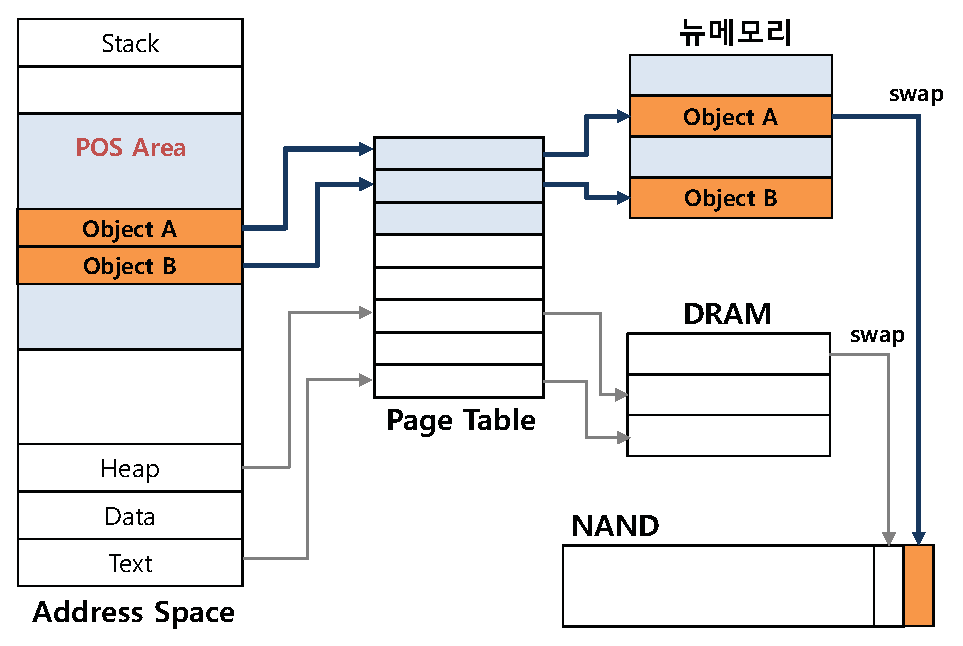
\includegraphics[width=3in]{./figure/swap_flow.eps}
\caption{NVM과 플래시 메모리 간의 스왑 동작}
\label{fig:swap_flow}
\end{center}
\end{figure}

\subsection{UFLRU: Unmapped-object First LRU}

리눅스의 기본 스왑 인/아웃 정책인 LRU에서 스왑 아웃 과정은, 추가적인 메모리의 확보를 위해서 Active/Inactive Page List의 페이지를 회수하는 작업을 진행한다. 이와 같은 페이지 회수 과정을 위해서는 Active/Inactive Page List의 페이지를 검사하여, 페이지의 회수가 가능한지 확인하는 작업이 필요하다. 검사 대상은 페이지의 더티 여부, 공유 여부, 그리고 참조 비트 등이며, 검사 결과에 따라서는 페이지의 회수를 위한 추가적인 작업이 필요한 경우가 생긴다. 이러한 추가적인 페이지의 처리 작업은 페이지 교체 작업의 시간을 더욱 증가 시켜, 스왑 인/아웃 정책의 성능 감소 원인이 된다. 때문에, 본 논문에서는 이러한 페이지에 대한 추가적인 처리 작업을 최소화 하는 것을 통해, 스와핑 정책의 효율을 향상 시키고자 하였다.

\subsubsection{UFLRU에서 스왑 아웃 페이지 선정 기준}

UFLRU에서 고려하는 페이지 처리 작업은 총 2가지가 있다. 그 중 하나는 페이지를 참조하는 프로세스의 페이지 테이블의 값을 수정하는 작업이다. 스왑 아웃 대상으로 선정된 페이지에 대해 하나 이상의 프로세스가 참조하는 경우, 페이지를 참조하는 모든 프로세스의 페이지 테이블 정보를 수정해야 한다. 이런 과정은 프로세스들에 대한 검색은 물론, 각각의 프로세스의 페이지 테이블을 변경하는 과정에서 상당한 시간적 비용이 발생하게 된다. 이를 방지하기 위해서, UFLRU는 페이지의 참조 여부를 가장 먼저 확인한다. 만약 페이지를 검사하였을 때 페이지를 참조하는 프로세스가 없는 경우에는, 프로세스의 순회 및 수정과 같은 작업이 필요 없기 때문에 스왑 인/아웃 작업의 속도를 단축할 수 있다. 때문에, UFLRU는 프로세스에 의해 참조가 되어있는 영속 객체보다, 참조되지 않은 영속 객체의 페이지의 스왑 아웃 선정 기준의 우선순위가 높다고 판단한다. 

UFLRU에서 고려할 또 다른 작업은 Dirty 페이지에 대한 Writing 작업이다. Dirty 페이지는 메모리에 기록 된 페이지의 내용이 저장 장치의 페이지의 내용과 서로 다른 경우에 발생하는 상황이다. 때문에, 해당 페이지를 스왑 대상으로 선정하기 위해서는, 메모리에 있는 페이지의 내용을 저장 장치의 스왑 파티션 영역에 기록하는 작업이 필수적이다. 이와 같은 페이지 처리 작업은 저장 장치에 접근하여 기록하는 작업이 포함되어 있기 때문에, 메모리에서 일어나는 작업보다 더욱 많은 시간 비용이 필요하게 된다. 반대로, Dirty 페이지가 아닌 경우는 저장 장치에 대한 접근이 필요 없이, 메모리 상에서 즉시 페이지를 회수할 수 있어 빠른 스왑 인/아웃 속도를 보장하게 된다. 때문에, UFLRU는 Dirty 페이지인 경우보다, Dirty 페이지가 아닌 경우의 영속 객체 페이지의 스왑 아웃 선정 기준 우선순위가 높다고 판단한다.

만약 페이지 리스트의 모든 페이지가 적어도 한 개의 프로세스에게 참조되었거나, Dirty 페이지만 존재하는 경우, 스왑 아웃 선정 기준은 기존 리눅스의 Swap In/Out 정책인 LRU 의거하여 페이지 리스트의 Tail 부분부터 순서대로 스왑 아웃 대상 페이지로 선정한다.  

\subsubsection{Active/Inactive Page List 정렬 방법}

\begin{figure}[t]
\begin{center}
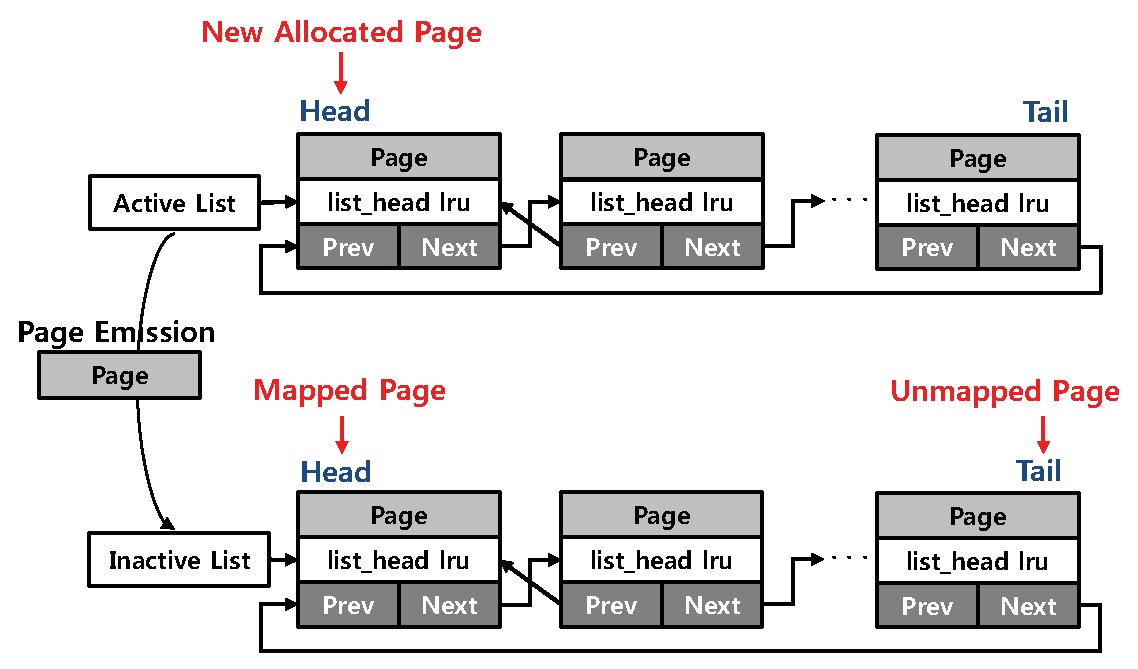
\includegraphics[width=3in]{./figure/uflru_list.eps}
\caption{UFLRU 페이지 리스트 관리 방법}
\label{fig:uflru_list}
\end{center}
\end{figure}

UFLRU에서 Active/Inactive Page List 정렬 방법은 그림 \ref{fig:uflru_list}과 같다. 먼저 새로 할당되거나 자주 사용된 페이지는 Active Page List의 Head에 삽입되며, 내부 페이지의 순서는 LRU 알고리즘으로 관리된다. 스왑 아웃 과정 중 Active Page List보다 Inactive Page List가 일정 비율보다 작을 경우에는, Active Page List의 페이지를 Tail부터 검사하여 Inactive Page List로 방출한다. 방출되는 페이지는 스왑 아웃 대상 페이지 선정 기준에 따라 Inactive list의 Head이나 혹은 Tail로 삽입될 지의 여부가 결정된다. 참조되었거나 Dirty 페이지의 경우에는 Inactive List의 Head로 삽입하며, 참조하는 프로세스가 없고 Clean 페이지인 경우에는 Inactive list의 Tail에 삽입한다. 이와 같은 과정을 통하여 Inactvie Page List의 Tail에는 페이지 처리 작업의 시간이 적게 걸리는 페이지들이 위치하며, Head에는 비교적 페이지 처리 작업의 시간이 오래 걸리는 작업들이 위치한다. UFLRU 알고리즘에서 스왑 아웃이 발생하게 될 때 메모리 회수 작업을 Inactve Page List의 Tail부터 실시하여 메모리를 확보한다. 따라서, 해당 과정을 통해서 페이지 리스트를 관리할 경우, 페이지 리스트의 Tail에는 상대적으로 매핑이 되지 않는 Clean 페이지들이 위치할 것이다. UFLRU는 이러한 페이지 관리 방법을 통해서 페이지 처리에 대한 시간적 비용을 감소시켜, 성능의 향상을 목표로 한다.

\subsubsection{스왑 아웃 중 페이지 처리 방법}
만약 스왑 아웃 과정에서 Inactive page list의 모든 페이지가 Dirty 페이지거나 매핑된 페이지일 경우, 기존 리눅스의 스와핑 정책처럼 페이지의 처리가 필요하게 된다. 

매핑 된 페이지의 경우, Reverse Mapping Tree 구조체에 페이지를 참고하는 프로세스들의 페이지 테이블 엔트리에 대한 정보를 기록하고 있다. 때문에, Figure 2처럼 페이지에 연결된 Reverse Mapping Tree를 선회하여, 페이지를 참고하는 프로세스의 페이지 테이블 엔트리를 스왑 엔트리로 변경하는 작업을 진행한다. 

\begin{figure}[h]
\begin{center}
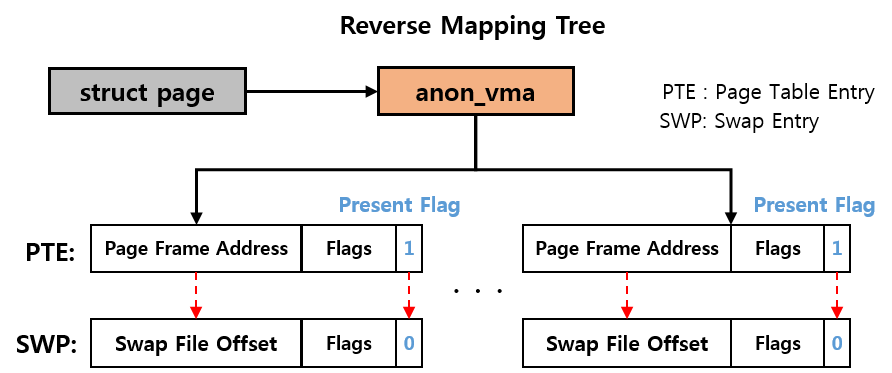
\includegraphics[scale=0.55]{fig2.png}
\end{center}
\caption{매핑된 페이지의 처리 방법}
\end{figure}

Dirty 페이지는 저장 장치에 페이지의 내용을 기록하는 도중에는 wirteback 플래그를 설정하며, 기록이 완료되면 PG\_reclaimable 플래그를 설정하는 작업을 실시한다. 만약, 페이지가 dirty이거나 writeback 플래그가 설정되어 있더라도, PG\_reclaimable이 설정되어 있다면 페이지는 clean 페이지처럼 회수가 가능하다. 

\subsection{스와핑 알고리즘 별 동작 예시}
\begin{figure}[h]
\begin{center}
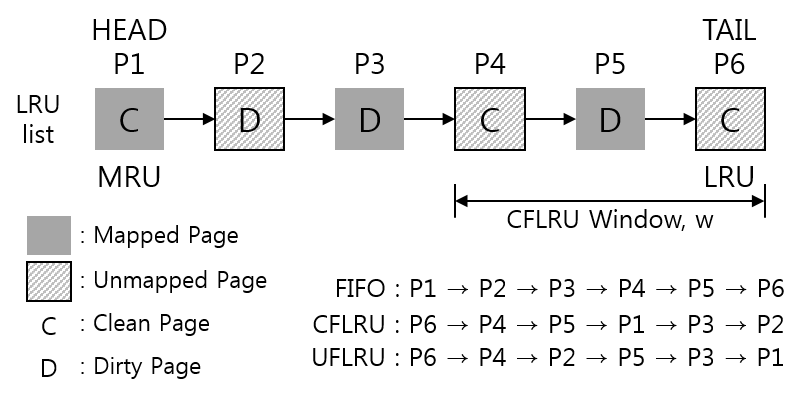
\includegraphics[scale=0.6]{fig3.png}
\end{center}
\caption{스와핑 알고리즘 별 동작 예시} 
\end{figure}
다음 Figure 3는 각 알고리즘에서의 스왑 아웃 과정 중, Inactive Page List의 스왑 아웃 페이지 선정 순서를 나타낸다.

먼저, FIFO의 경우에는 다음과 같이 리스트에 삽입된 순서인, P1 → P2 → P3 → P4 → P5 → P6의 순서로 스왑 아웃 페이지를 선정하게 된다. 이와 같은 작업은 매핑 유무와 Dirty 유무를 상관 하지 않기 때문에, 예시와 같은 페이지 리스트에서 최악의 실행 시간을 보여준다. 

CFLRU의 경우 CFLRU window 내부에 있는 페이지들을 먼저 검사하여, Clean 페이지를 먼저 내리는 작업을 진행한다. 때문에, P6 → P4 → P5 → P1 → P3 → P2의 순서로 페이지 스왑 아웃 대상을 선정하는 것을 알 수 있다. 이러한 과정은 FIFO보다 Dirty 페이지를 처리하는 과정에서 충분히 빠른 속도를 보장하지만, 매핑 된 페이지에 대한 처리에서 추가적인 시간이 발생하기 때문에 최적화 된 방법은 아니다. 

UFLRU의 경우, 매핑 여부와 Dirty 여부를 동시에 고려하므로, P6 → P4 → P2 → P5 → P3 → P1의 순서로 스왑 아웃 대상 페이지를 선정하게 된다. 이러한 방법의 경우, Dirty 페이지의 처리 시간은 물론, 매핑 된 페이지에 대한 처리 시간 또한 감소하게 된다. 때문에,  위에서 소개된 3가지의 알고리즘 중, UFLRU가 가장 좋은 성능을 보여줄 수 있다.

\section{성능 평가}
\subsection{실험 환경(Experiment Setup)}
본 논문에서는 스와핑 실험을 위해 1 Gbyte의 DRAM 메모리와 512 Mbyte NVRAM를 할당하였으며, 스왑 파티션 영역의 크기는 18 GBytes로 설정하였다. 또한, NVRAM 영역에서의 스와핑 동작을 확인하기 위해서, 영속 객체를 NVRAM이상의 크기로 생성할 필요가 있다. 때문에, 400개의 프로세스가 각각 2 MByte씩 영속 객체를 생성하여, 총 800 MByte의 영속 객체를 생성 한다. 이 후, 임의의 객체에 접근하여 객체의 모든 데이터를 업데이트하는 동작을 통해 스와핑 알고리즘의 성능을 평가하고자 하였다. 모든 실험은 Intel i7 (920) 2.67 GHz CPU, WD 1 TByte 7,200 RPM HDD, Linux 3.15 커널 기반에서 실시하였다.

UFLRU의 성능을 비교 평가하기 위해 여러가지의 희생 페이지 선정 알고리즘를 구현할 필요가 있다. 때문에, Linux 3.15 커널에 default로 적용되어 있는 스와핑 알고리즘인 Second Chance LRU (SCLRU)는 물론, First-In First-Out (FIFO), Clean-First LRU (CFLRU)과 같은 희생 페이지 선정 알고리즘을 구현하여, 동일한 워크로드에서 각 알고리즘의 성능을 측정하였다.

\subsection{워크로드}

프로세스가 영속 객체를 생성할 때, 각 객체들을 빈번하게 접근되는 Hot 객체와 간헐적으로 접근되는 Cold 객체로 구분하였다. Hot 객체의 접근 빈도는 전체 객체 접근의 80\%를 차지하며, Cold 객체보다 더 많은 접근이 일어난다. Hot 객체의 수는 전체 영속 객체에서 10\%, 20\%, 30\%, 40\%, 50\%의 비율로 생성하도록 하였으며, Hot 객체의 비율에 따른 실험 결과를 측정하였다.

\subsection{실험 결과}

\begin{figure}[h]
\begin{center}
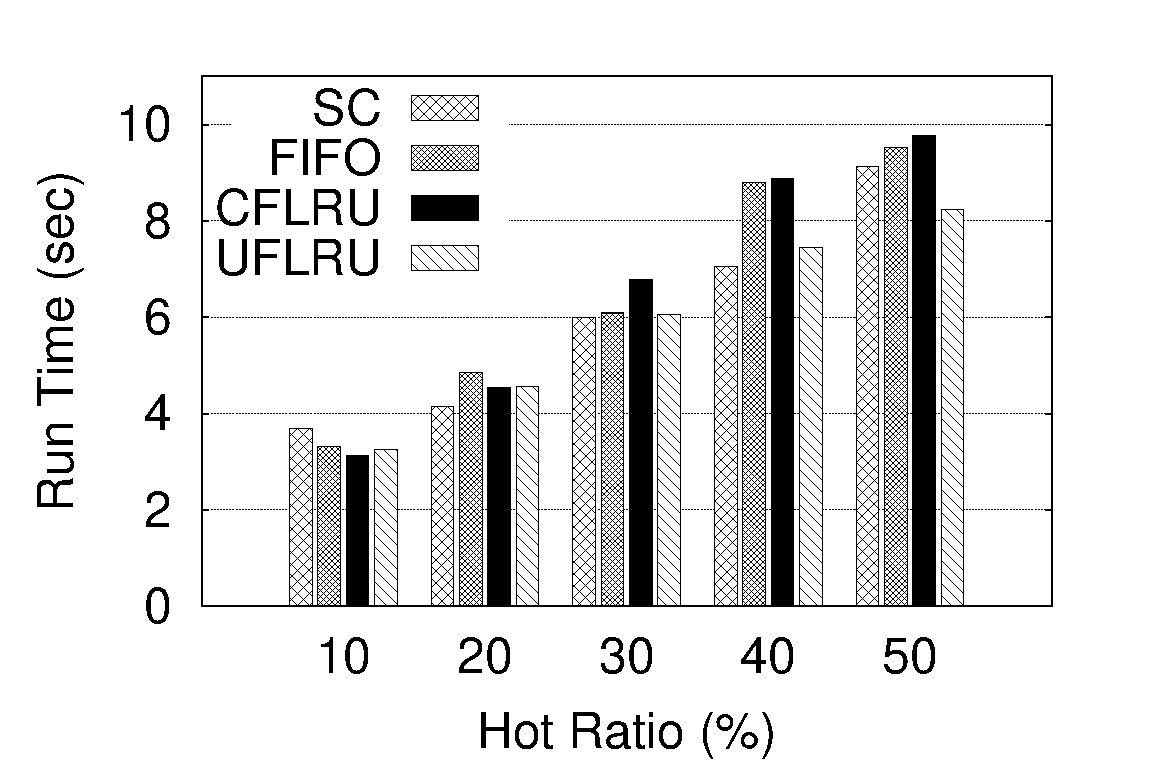
\includegraphics[width=3in]{./figure/exe_time.eps}
\caption{희생 페이지 선정 알고리즘 별 실행시}
\label{fig:exe_time}
\end{center}
\end{figure}

그림 \ref{fig:exe_time}은 Hot 객체의 비율을 10\%에서 50\%로 증가시켰을 때, 워크로드의 총 실행시간을 보여주며, Hot 객체의 비율이 많아질수록, 스왑 아웃 동작이 자주 발생함을 확인할 수 있다. 그에 따라 테스트 수행시간 또한 Hot 객체 비율이 커질수록 약 3초에서 9초로 3배 증가하였다. 특히 Hot 객체 비율이 50\%인 워크로드에서는 UFLRU의 실행 시간이 CFLRU 대비 15\% 감소함을 확인하였다.

\begin{figure}[h]
\begin{center}
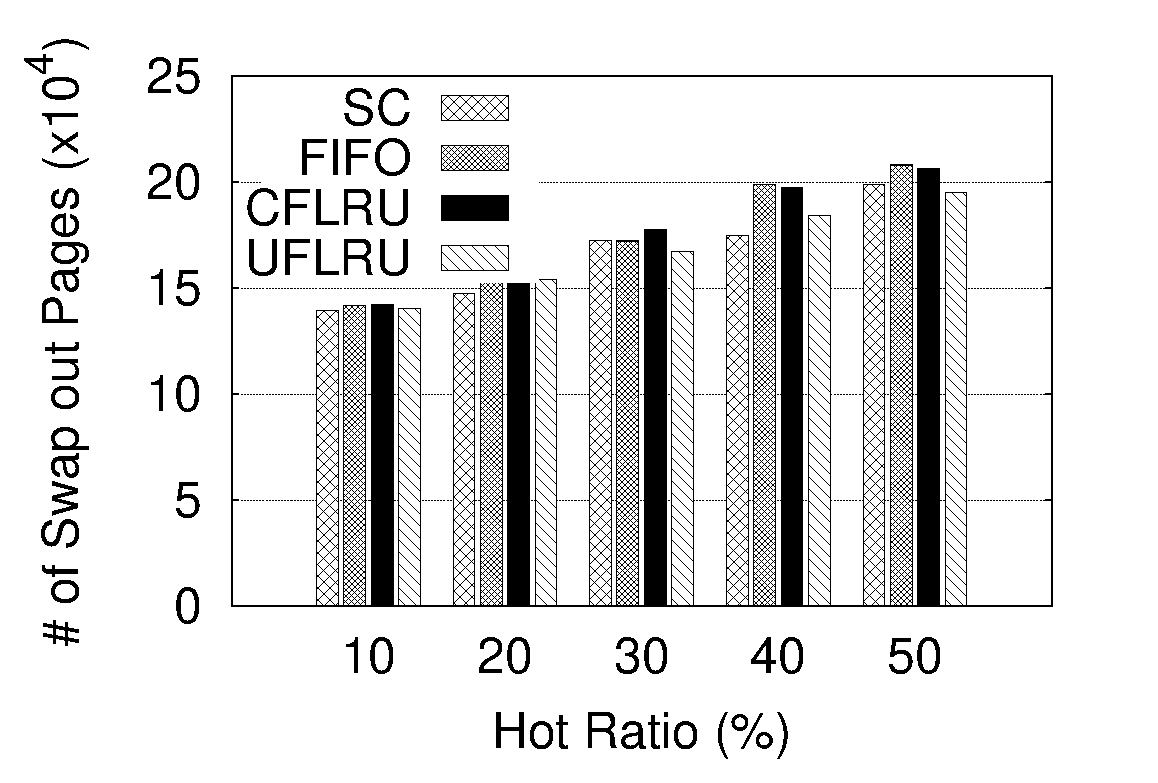
\includegraphics[width=3in]{./figure/swap_count.eps}
\caption{희생 페이지 선정 알고리즘 별 스왑아웃 페이지 수 비교}
\label{fig:swap_count}
\end{center}
\end{figure}


그림 \ref{fig:swap_count}는 각 실험에서 Hot 객체의 비율을 10\%에서 50\%로 증가시켰을 때, 스왑 영역으로 스왑 아웃 된 페이지의 수를 보여준다. 실행 시간의 경우와 마찬가지로 Hot 객체의 비율이 증가함에 따라 스왑 아웃 된 페이지의 수가 증가한다. 실행시간 그래프와 비교하여, 전체 스왑 아웃된 페이지의 수가 비슷하지만 실행 시간에는 차이가 있는 경우가 존재하는 것을 볼 수 있다. 특히, UFLRU의 경우 스압 아웃된 페이지의 수가 다른 알고리즘과 비슷한 경우라도 실행 시간이 낮음을 볼 수 있는데, 이러한 경우는 각 알고리즘 별로 스와핑 과정에 대해서 전체 스왑 아웃된 페이지의 수는 같지만, UFLRU의 경우에는 개별 페이지에 대한 처리 및 검사에 대한 시간이 줄어들었기 때문이다.

\section{관련 연구}

Mnemosyne는 영속 객체를 생성 및 관리하기 위해, 유저 Library 영역과 커널 영역을 가진다. 유저 Libraray에는 Durable Transactions, Persistence Primitives, 그리고 Persistent Regions가 있다. 커널 영역에는 Region Manager layer를 두어 유저 영역에서의 요청을 처리하도록 하였다. Mnemosyne의 이러한 구조의 장점은 데이터의 Transaction 단위 처리가 가능하다는 점, Logging을 통한 Recovery mechanism를 지원한다는 점이 있다. 

이를 통해 Mnemosyne은 데이터의 atomicity를 보장 할 수 있지만, 공유 메모리 환경에서는 문제가 발생할 수 있다. 공유 메모리에 크래시가 발생하여 Recovery mechanism을 하여야 한다고 가정하자. Mnemosyne이 Logging 과정을 통해서 데이터를 복원할 때, 해당 Logging 내용의 주체가 되는 프로세스를 알 수 없다. 때문에, 복원된 데이터와 원본 데이터 간의 Inconsistency가 발생할 수 있다는 문제점이 발생한다. 이를 해결하기 위해서 Mnemosyne 논문에서는 공유 프로세스 중 1개만이 logging을 하거나, 프로세스가 공유 메모리에 접근하기 전 Recovery mechanism을 실행하고 완료하는 방법을 제시하였다. 하지만, 이와 같은 제약은 공유 메모리를 자주 사용하는 리눅스의 현 정책 상 상당한 성능 저하를 일으킬 요소가 되며, 때문에 본 논문에서는 Mnemosyne를 사용하지 않기로 결정하였다. \cite{volos2011mnemosyne}.

또 다른 비휘발성 메모리 관리 프로그램인 HEAPO는 프로세스에게 영속 객체에 대한 관리 및 공유를 위한 high-level 인터페이스를 제공하는 프로그램이다. HEAPO는 영속 객체에 대한 HEAPO 내부에서 관리하는 메타데이터를 통해서, 영속 객체의 가상 주소 영역과 비휘발성 메모리의 물리 주소 영역을 1:1로 관리한다. 이와 같은 HEAPO의 메모리 관리 방법은, HEAPO의 인터페이스 이외의 영속 객체에 접근을 차단하여 영속 객체에 대한 보호 및 관리를 가능하게 한다. 또한, 프로세스가 수정한 내용은 HEAPO 내부의 메타데이터에 관리되기 때문에 공유 메모리의 경우에도, 데이터의 Inconsistency가 발생하지 않는다.

CFLRU (Clean-First LRU)는 기존 리눅스의 LRU 정책에서 한 단계 더 나아가, 스왑 아웃 과정 중 페이지의 Dirty 유무를 고려하여 스왑 아웃 대상 페이지를 선정하는 알고리즘이다. 기존 리눅스에서는 Inactive list의 Tail부터 페이지에 대한 처리를 차례로 진행하는 반면, CFLRU는 CFLRU Window의 Tail부터 페이지를 검사할 때, 페이지가 Dirty라면 무시하고 다음 페이지를 검사한다. 이와 같은 알고리즘의 장점은 Inactive list의 내부에 Clean 페이지가 상당수 존재하는 경우, 기존 리눅스의 정책보다 더욱 빠른 작업 시간을 보장할 수 있다는 점이다.

하지만, Inactive list의 모든 페이지가 Dirty인 경우에는 결국 기존 리눅스의 동작과 다를 바 없으며, 무엇보다 CFLRU Window를 2번 순회해야하는 오버헤드가 발생하게 된다. CFLRU의 알고리즘의 특성 상, 메모리가 부족하여 일어나는 스왑 아웃 과정에서 Inactive list의 모든 페이지가 Dirty 페이지일 가능성은 매우 높게 되며, 매핑 페이지에 대한 고려가 없으므로 그에 따른 오버헤드 또한 발생할 수 있다는 문제점이 있다 \cite{park2006cflru}. 

Conquest는 NVRAM과 저장 장치를 동시에 사용하여 파일의 내용을 기록할 수 있는 NVRAM 기반의 파일 시스템이다. 먼저, Conquest는 파일의 크기가 상대적으로 작으면 NVRAM에 파일 데이터 및 메타데이터를 저장한다. 반대로, 상대적으로 파일의 크기가 큰 경우에는 파일의 내용을 하드 디스크에 순차적으로 기록하며, 파일에 대한 메타데이터, 실행파일, 그리고 공유 라이브러리는 NVRAM에 저장한다. 이러한 구조는 파일의 크기가 적은 경우가 큰 파일의 경우보다 데이터의 접근이 많다는 점에 착안한 디자인이다. 즉, 파일 접근이 많은 경우는 NVRAM에 그 내용을 저장하도록 하고, 반대로 파일 접근이 적은 경우에는 하드 디스크에 그 내용을 기록하는 방식을 사용하여 시스템의 성능을 올릴 수 있는 방법이다 \cite{wang2002conquest}.  

하지만, 큰 파일의 데이터의 접근이 작은 파일보다 적다고 하더라도, 큰 파일의 내용을 일부분이라도 읽어오기 위해서는 하드 디스크에 접근해야 한다는 단점이 존재한다. 게다가, 큰 파일이 자주 쓰이는 경우가 많은 시스템이나 대용량 파일이 많은 미디어 환경에서는 일반적인 파일 시스템에 비해, 하드 디스크에서 데이터를 자주 읽어와야 하는 오버헤드가 발생하는 문제가 있다. 또한, 낸드 플래시에서의 동작을 상정하고 있지 않기 때문에, 저장 장치로 낸드 플래시 메모리를 사용하는 환경에서는 성능 감소가 일어날 수 있다 \cite{huang2014tridentfs}.

TridentFS 역시 Conquest와 마찬가지로 NVRAM을 사용할 수 있는 파일 시스템이지만, Conquest와 달리 낸드 플래시 메모리는 물론 하드 디스크에 대한 데이터의 저장 방식도 고려하고 있는 하이브리드 파일 시스템이다. TridentFS는 파일의 inode flag를 통해서 NVRAM, 낸드 플래시 메모리, 그리고 하드 디스크 중 파일의 내용을 저장된 곳을 구분하는 방식을 사용한다. 또한, 만약 NVRAM의 메모리를 모두 사용하더라도, NVRAM 데이터를 하드 디스크와 낸드 플래시 메모리로 스왑 아웃 하는 동작을 실시하여 추가적인 메모리를 확보한다.  
문제는 inode로 관리되지 않는 영속 객체의 경우에는 영속성을 보장할 수 없으며, 스압 아웃된 NVRAM의 데이터를 찾기 위해서 하드 디스크와 낸드 플래시 메모리를 검색하는 과정을 거쳐야 한다. 게다가 NVRAM의 페이지의 스왑 아웃 과정 중 크래시가 날 경우, NVRAM 메타 데이터와 파일 데이터 간의 Inconsistency가 발생할 수 있다는 문제가 발생한다. 또한, 현재 TridentFS에서는 스왑 아웃 된 NVRAM 데이터가 스왑 인 과정을 통해 다시 NVRAM에 기록되지 못하는 문제가 있다. 때문에, 영속성을 보장해야할 데이터가 스와핑 과정 이후에는 영속성이 보장되지 않게 되는 문제가 발생한다. 때문에, 본 논문에서는 TridentFS에서 구현한 스와핑 방식과는 다른 방식으로 스와핑을 구현할 필요성을 느끼게 되었다.


\section{결론}

본 논문에서 개발한 UFLRU 알고리즘은 비휘발성 메모리에 여유 공간이 부족할 때, 객체 매핑 여부 및 페이지의 Dirty 여부를 고려하여 스왑 대상 페이지를 선정한다. 그 후 선정된 스왑 대상 페이지는 플래시 메모리의 스왑 파티션 영역으로 방출하여 추가적인 메모리를 확보하는 기법이다. 제안한 알고리즘은 본 논문에서 고려한 스와핑 실험을 통한 성능 평가 결과, CFLRU 알고리즘 대비 15\%의 성능 개선을 보였다.

{\footnotesize \bibliographystyle{acm}
\bibliography{./uflru.bib}}


\end{document}






